% Chapter 1

\chapter{Some Basic Simulations} % Main chapter title

\label{Chapter1} % For referencing the chapter elsewhere, use \ref{Chapter1} 

\lhead{Chapter 1. \emph{Chapter Title Here}} % This is for the header on each page - perhaps a shortened title

%----------------------------------------------------------------------------------------


While the introduction outlined the computer programming necessary to produce simulations in general, this chapter will start to deal with the physics necessary to make simulations seem realistic.  In this chapter, I will outline some examples of simulations with balls bouncing, and discussing the basic mechanics involved through the code.



\section{Basic Ball Bouncing}

A ball bouncing will show the basic kinematic equations, and how they are used in the javascript code.  The following example displays a ball being dropped with an initial $v_x$, and bouncing off the walls and floor of the canvas element.  The full code is shown below:




\setstretch{1}
\begin{lstlisting}[breaklines=true, frame=single, numbers=left, caption=A basic ball bouncing simulation, label=lst:ballbounce1]
var canvas = document.getElementById(`canvas');
var context = canvas.getContext(`2d'); 

canvas.height = screen.height-200;
canvas.width = screen.width -100;

var radius = 20;
var color = ``red";
var g = .1635; // acceleration due to gravity
var x = 40;  // initial horizontal position
var y = 40;  // initial vertical position
var vx = parseFloat(prompt(`what is the initial horizontal speed of ball you would like?(recommended values of 1-20'));  // initial horizontal speed 
var vy = 0;  // initial vertical speed
 
window.onload = init; 
 
function init() {
  setInterval(onEachStep, 1000/60); // 60 fps
};
 
function onEachStep() {
  vy += g; // gravity increases the vertical speed
  x += vx; // horizontal speed increases horizontal position 
  y += vy; // vertical speed increases vertical position

  if (y > canvas.height - radius){ // if ball hits the ground
    y = canvas.height - radius; // reposition it at the ground
    vy *= -0.8; // then reverse and reduce its vertical speed
  }
  if (x > canvas.width - radius){ // if ball hits right wall
    x = canvas.width - radius; // reposition it right at wall 
    vx *= -0.8;  // then reduce and reverse horizontal speed
  }
  if (x < radius){  // if ball hits left wall
    x = radius;  // reposition it right at wall
    vx *= -0.8  // then reverse and reduce horizontal speed
  }
  drawBall(); // draw the ball
};
 
function drawBall() {
  with (context){
    clearRect(0, 0, canvas.width, canvas.height); 
    fillStyle = color;
    beginPath();
    arc(x, y, radius, 0, 2*Math.PI, true);
    closePath();
    fill();
  };
};

\end{lstlisting}
\setstretch{2}

This code functions by first setting up the canvas to be an appropriate size, on lines 1-5.  Then, the simple variables of radius, color, initial positions/velocities, and acceleration are initialized.  As mentioned in the introduction, the canvas HTML element defines positions in terms of pixels, with the top left corner of the canvas being the origin.  Therefore, the ball is initialized to appear at (40, 40) which is near the top left corner for any computer screen.  The value of g, the gravitational constant, is set to .1635 to accurately represent its value near Earth's surface, of $9.81 \hspace{1mm} \frac{m}{s^2}$.  To understand why this value makes sense, it is necessary to understand the units of velocity on the HTML canvas.  The position during the simulation is given in terms of pixels, which of course differs from the SI unit of meters.  However, as long as g can be initialized to be $9.81 \hspace{1mm} \frac{px}{s^2}$, the simulation will still look physically accurate.  This can be explained with the equation below:

\begin{equation} \label{eq:pixelsconversion}
9.81 \hspace{1mm}  \frac{px}{s^2}  = .1635 \hspace{1mm}  \frac{\frac{px}{s}}{frame} \hspace{1mm}  \times \hspace{1mm}  \hspace{1mm}  \frac{60 frame}{s}
\end{equation}


The value of g is calculated based on the fact that the simulation was run at 60 frames per second.  Time is a central component of all physics, and for the simulations to behave realistically they must carefully take that into account.  

The remainder of the code involves 3 functions that call one another to create the flow of the simulation.  The first function, init (``initialize'') is called when the browser window is loaded(line 15).  This function simply delays the next function, onEachStep, by 16.66 ms, meaning that the function essentially runs 60 times per second, producing the desired 60 frames per second.  Line 18 accomplishes this in a crude method: simulations later will involve more sophisticated techniques.  The onEachStep function contains the instructions for each frame of the simulation.  It involves multiple conditional if-statement loops that create the illusion that the ball bounces off of the walls and floor.  

All 3 conditional loops involve a coefficient of restitution, or $C_r$.  This is a mechanical property, representing how ``bouncy'' the ball is, and measures the ratio of the kinetic energy after and before the impact.  This is derived below:

\begin{equation}\label{eq:cr}
C_r = \sqrt{\frac{KE_f}{KE_i}} = \sqrt{\frac{\frac{1}{2} mv_f^2}{\frac{1}{2} mv_i^2}} = \frac{v_f}{v_i}
\end{equation}

A $C_r$ value of .8 was used for this simulation, which is comparable to that of a tennis ball\textsuperscript{\cite{tennisball}}.  The variable Cr represents this value in the code, and is simply multiplied by the velocity before impact, so the following equation results:

\begin{equation}\label{eq:velocitycr}
v_f = v_i * C_r
\end{equation}

An essential part of any physics simulation involves \textit{collision detection}.  For the simple bouncing ball simulation, this is accomplished by conditional loops for if the ball's position exceeds the canvas constraints.  


The last function of the program, drawBall, simply contains commands for the canvas API to draw.  While these commands can be very complicated and intricate to create the exact visual aesthetic desired, the extent of these commands is not the purpose of this thesis.  Basically, this function works by ``erasing'' the canvas of any previous graphics, and then creating a new visual with the arc() method.   

The logic of the program can be summarized through the flow chart below:


\begin{figure}[h] 
	\centering
		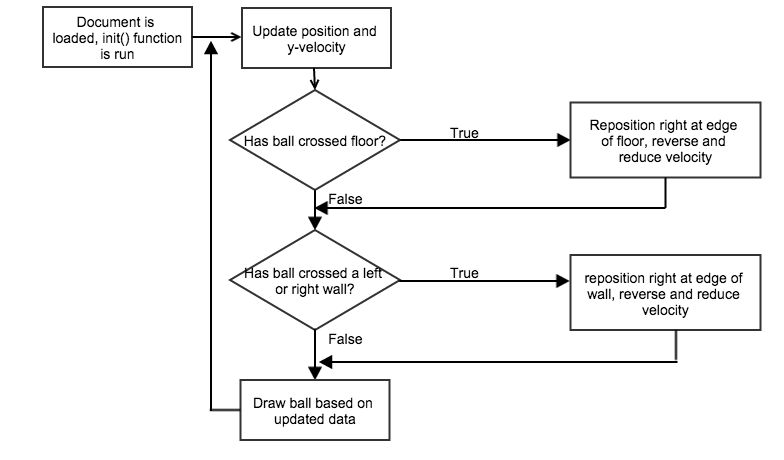
\includegraphics[width=15cm]{Figures/basicbouncingball.png}

	\caption{The logic flow chart of the basic bouncing ball simulation}
	\label{fig:basicbouncingball}
\end{figure}




\section{More Advanced Ball Bouncing}

While the previous example realistically incorporated the basic kinematic equations into account, it still fails to recognize important fundamentals of physics.  The simulation in this chapter will still be a simple ball bouncing, but will take into account air resistance.

\subsection{Background Physics}

Drag is generally defined as the force on an object that resists its motion through a fluid.  In the case of air resistance, the fluid is a gas, and therefore the process is called aerodynamic drag.  Most of the drag force results as a response to the inertia of the fluid: the resistance it exerts to oppose being pushed aside.  This can be expressed in the equation below:

\begin{equation} \label{eq:drag}
f_{drag} = -\frac{1}{2}C_d \rho A v^2
\end{equation}

The equation involves a negative sign because the force of drag is always opposite the direction of motion.  $C_d$ is referred to as the drag coefficient, and is a dimensionless quantity that is used to model complex dependencies of shape, inclination, and flow conditions.  While $C_d$ is in general not an absolute constant for a given body shape, for the purpose of these simulations constant values were used.  These values are typically determined experimentally: for example, the $C_d$ of a sphere is approximately .47.  In equation \ref{eq:drag}, $\rho$ is the mass density of the fluid, in $\frac{kg}{m^3}$.  Most of the simulations in this thesis occur in air, which has a density of 1.225 $\frac{kg}{m^3}$  (at sea level and 15 \textdegree C).  Running the simulations in different fluids can be simulated by changing $\rho$ to higher values (water, for example, would have $\rho$ equal to 1000 $\frac{kg}{m^3}$).  Lastly, $A$ in equation \ref{eq:drag} is the cross-sectional area of the object.  A sphere, for example, would have a cross-sectional area of $\pi r^2 $ 

The basic kinematic equations can also be used to make the simulations more physically realistic.  

\begin{equation}\label{eq:position}
d = v_i t+ \frac{1}{2}at^2
\end{equation}
\begin{equation}\label{eq:v}
v_f = v_i + at
\end{equation}

These equations are fundamental to any physical situation and can be used to make the ball bouncing example of the previous section more realistic

\subsection{The Code}

Using these basic mechanics equations, the previous ball bouncing example can be made more physically accurate.  The code below shows a second simulation which incorporates air resistance:

\setstretch{1}
\begin{lstlisting}[breaklines=true, frame=single, numbers=left, caption=More advanced ball bouncing simulation, label=lst:ballbounce2]
var x = 40;
var y =40;
var vy = 0;
var ay = 0;
var m = 1;
var r = 20;
var rSI = r* 0.000230909;  // radius in SI, converting px to m
var C_r = .8;  // Coefficient of restitution (tennis ball would be .8)
var rho = 1.2;    // density of air would be 1.2, water would be 1000
var dt = 60/1000;  // Time Step
var C_d = 0.47; //Coefficient of drag for sphere
var A = Math.PI * rSI * rSI;
var color = 'red';

window.onload = init();
  
function init(){
  setInterval(onEachStep, 1000/60);
}

function onEachStep(){ 
  var fy = 0;
  fy += m * 9.81;   // weight force
  if (vy>=0){
    fy -= 1* 0.5 *rho * C_d *A *vy *vy; 
  } 
  else {
    fy += 1*0.5 *rho *C_d *A *vy *vy;
  }

  ay = fy / m;
  vy += ay * dt;
  y += vy;
  
  // simple collision detection for floor only
  if (y + r > canvas.height){ 
    vy *= -C_r; 
    y = canvas.height - r;  
  }
  drawBall();
}
\end{lstlisting}
\setstretch{2}

To eliminate redundancy, the code doesn't show previous functions used, such as drawBall().  The code also doesn't show the basic steps to initialize any simulation with the canvas and context commands.  The code is very similar to the simulation in the previous section, except it incorporates air resistance.  Essentially, this simulation uses more kinematic equations, by calculating the net force, acceleration, and velocity for each frame.  First, the net vertical force is caculated, by combining the force of gravity $F_g = mg$ with the air drag from equation \ref{eq:drag}.  This step involves a conditional loop for the cases of positive and negative velocity.  Once the net force is calculated, the acceleration in the y-direction is found by using Newton's 2nd law of $F = ma$.  From there, the velocity and vertical position of the ball are updated.  Unlike the previous simulation, this example involves a variable dt, which is set to $\sim$16 ms for the same 60 frames per second.   


This code involves interesting conversions between pixels and meters.  Becuase the on screen simulation is presented eventually in terms of pixels, the physics equations must acknowledge this.  The variable rSI on line 7 converts the radius of ball from pixels into meters.  This is accomplished knowing the pixel density of the screen.  This is commonly approximately 100 (dots per inch).  The simulations were optimized for a macbook pro 15 inch model, which features 110 dpi.  The calculation is shown below:

\begin{equation}\label{eq:pixels}
\frac{1m}{100 cm} \hspace{1mm} \frac{2.54 cm}{1 in}  \hspace{1mm}   \frac{1 in}{110 px} \approx  0.00023091 \frac{m}{px}
\end{equation}

Once the conversion is made, the physics equations use the radius of the ball in terms of meters instead of pixels, which would give erroneous answers.

\section{Multiple Balls Bouncing}

So far, this chapter has dealt with a single object in motion.  However, physics rarely involves just one body in motion.  To demonstrate how more than one object can be displayed simultaneously, this section will show the case of multiple bouncing balls.  There is no new physics introduced in this section, but the coding concepts will be used repeatedly in later chapters of this thesis.

\subsection{The Code}

To generate more than one object, arrays can be used.  The code below relies on arrays and object prototypes to create the effect:

\setstretch{1}
\begin{lstlisting}[breaklines=true, frame=single, numbers=left, caption=Multiple balls bouncing simulation, label=lst:ballsbouncing]
var g = 0.1635;
var balls;
var numBalls = prompt('how many balls would you like to have bounce?'); 
var C_d = .8;
 
window.onload = init; 
 
function init() {
  balls = []; // creates empty array
  for (var i=0; i<numBalls; i++){
    radius = Math.random()*20+5;
    var ball = new Ball();  
    ball.x = 50;
    ball.y = 75;
    ball.radius =  radius;
    ball.vx = Math.random()*15;
    ball.vy = (Math.random()-0.5)*10;
    ball.color = getRandomColor();
    ball.draw(context);
    balls.push(ball);
  }  
  setInterval(onEachStep, 1000/60); // 60 fps
};
 
function onEachStep() {
  context.clearRect(0, 0, canvas.width, canvas.height); 
  for (var i=0; i<numBalls; i++){
    var ball = balls[i];
    ball.vy += g;     

    if (ball.vx >0){ // while vx is positive, decrease to show friction/air drag
    ball.vx -= .001;
  } else{
    ball.vx === 0;// make sure ball stops moving appropriately
  }
    ball.x += ball.vx; 
    ball.y += ball.vy; 
      
    if (ball.y > canvas.height - ball.radius){ 
      ball.y = canvas.height - ball.radius; 
      ball.vy *= -C_d; 
    }
    if (ball.x + ball.radius > canvas.width){
      ball.x = canvas.width - ball.radius; 
      ball.vx *= -C_d;
    }
    if (ball.x < ball.radius){
      ball.x = ball.radius;
      ball.vx *= -C_d;
    }
    ball.draw(context); 
  } 
};

function getRandomColor() {
    var letters = '0123456789ABCDEF'.split('');
    var color = '#';
    for (var i = 0; i < 6; i++ ) {
        color += letters[Math.floor(Math.random() * 16)];
    }
    return color;
}
\end{lstlisting}
\setstretch{2}


As with previous code listings, steps outlined in previous examples have been omitted to save space.  This code differs mainly from previous examples because of its usage of prototypes, objects, and arrays.  A separate javascript file, ball.js, contains the framework code for creating a ball.  This will be used more in future chapters, so the code doesn't have to be repeated.  This function is called a constructor function, becuase it allows other parts of code to reference the function when creating a new object.  In the case of listing \ref{lst:ballsbouncing}, an array holds an object for each different ball generated.  The number of elements in the array is equal to the number of balls, which is selected by the user through the prompt() method on line 3.  The object in each array element contains different properties for each ball: the radius, color, position, and velocities.  For every frame of the simulation, a loop cycles through each element of the balls array, changing the properties of position and velocity, on lines 29 and 36-37.  Exactly like in section 1, there is a conditional loop that controls the event of the ball colliding with a wall.  The logic of this program can be visualized in the flow chart of figure \ref{blah}.

Because of repeated for loops, this program involves a bit more complexity than the previous examples.  However, the physics is very simple in this case.  Future chapters will combine more complex physics with this complexity of coding to create more advanced simuations.  These simulations can put a strain on a computer's performance: to simulate 20 balls bouncing, at 60 frames per second, 4,800 individual properties of objects need to be generated each second.  Luckily, with the modern capabilities of computers, this isn't too difficult.  

This program involves each ball having a random color and radius, when the balls array is created in the init() function.  The Math.rand() method is used for both of these, and is fundamental to the other simulations in this thesis.  The random color generator function operates by creating a hex color by randomly assigning the 16 possible entries to each entry of the 6 character string.  While completely unnecessary, this gives the program aesthetic appeal, and makes it easier to distinguish the balls.

\begin{figure}[t]  
  \centering
  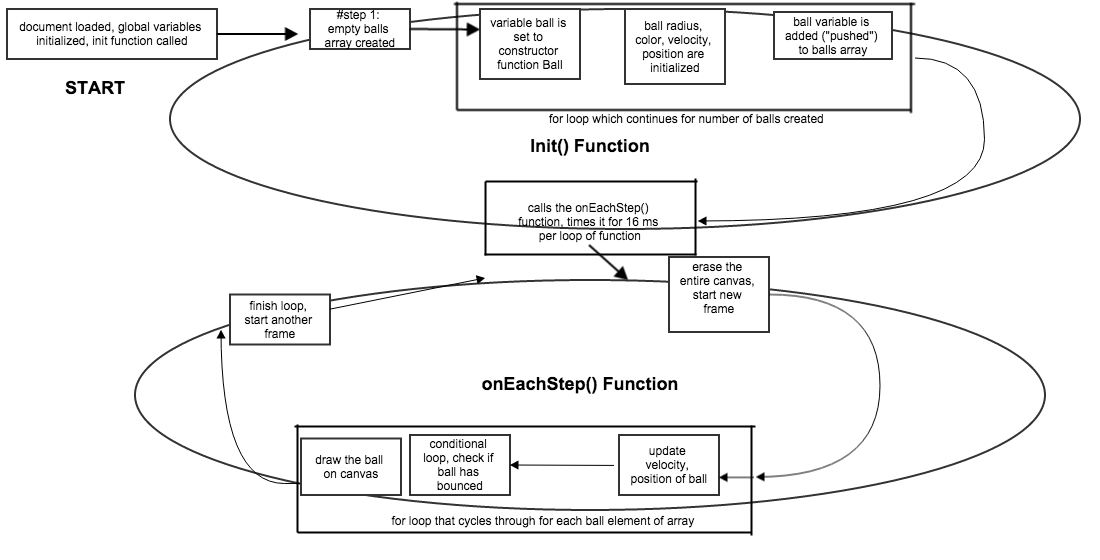
\includegraphics[width=15cm]{Figures/ballsbouncing.png}
  \caption{The logic flow chart of the balls bouncing simulation}
  \label{blah}
\end{figure}





































